\documentclass{report}
\usepackage[T1]{fontenc} % Fontes T1
\usepackage[utf8]{inputenc} % Input UTF8
\usepackage[backend=biber, style=ieee]{biblatex} % para usar bibliografia
\usepackage{csquotes}
\usepackage[portuguese]{babel} %Usar língua portuguesa
\usepackage{blindtext} % Gerar texto automaticamente
\usepackage[printonlyused]{acronym}
\usepackage{hyperref} % para autoref
\usepackage{subcaption}
\usepackage{graphicx}
 


\bibliography{bibliografia}


\begin{document}
%%
% Definições
%
\def\titulo{Sistema GIT}
\def\data{5-11-2019}
\def\autores{João Gameiro, Marco Ramos}
\def\autorescontactos{(93097) joao.gameiro@ua.pt, (93388) msramos99@ua.pt}
\def\versao{VERSAO}
\def\departamento{DETI - MPEI}
\def\empresa{UA}
\def\logotipo{ua.pdf}
%
%%%%%% CAPA %%%%%%
%
\begin{titlepage}

\begin{center}
%
\vspace*{50mm}
%
{\Huge \titulo}\\ 
%
\vspace{10mm}
%
{\Large \empresa}\\
%
\vspace{10mm}
%
{\LARGE \autores}\\ 
%
\vspace{30mm}
%
\begin{figure}[h]
\center
\includegraphics{\logotipo}
\end{figure}
%
\vspace{30mm}
\end{center}
%
\begin{flushright}
\versao
\end{flushright}
\end{titlepage}

%%  Página de Título %%
\title{%
{\Huge\textbf{\titulo}}\\
{\Large \departamento\\ \empresa}
}
%
\author{%
    \autores \\
    \autorescontactos
}
%
\date{\data}
%
\maketitle

\pagenumbering{roman}


%%%%%%%%%%%%%%%%%%%%%%%%%%%%%%%%
%%%%%%%%%%%%%%%%%%%%%%%%%%%%%%%%


\chapter{Introdução}
\label{chap.introducao}

O principal objectivo deste relatório é ajudar na percepção do código desenvolvido, explicar o funcionamento da aplicação concebida e outras eventuais questões relativas ao projeto desenvolvido no âmbito da unidade curricular de \ac{mpei}, do curso \ac{ect}.

A aplicação constitui uma espécie de simulação do que poderia ser um Sistema Git para armazenamento de ficheiros. As funcionalidades da mesma incluem:
\begin{itemize}
   \item Adição de ficheiros;
   \item Remoção de ficheiros;
   \item Pesquisa e listagem de ficheiros;
   \item Procura de similaridade entre ficheiros.
 \end{itemize}
 
 A aplicação foi desenvolvida usando a linguagem de programação {\itshape Java} e é composta por vários componentes, que serão explicitados nos capítulos à frente.

Este documento está dividido em quatro capítulos.
Depois desta introdução,
no \autoref{chap.app} são apresentados todos os constituintes da aplicação,
no \autoref{chap.test} são expostos e analisados os testes realizados enquanto que o \autoref{chap.func} refere-se ao funcionamento da aplicação.
Finalmente, no \autoref{chap.conclusao} é apresentada uma visão geral do trabalho acompanhada de uma conclusão sobre o mesmo.


%%%%%%%%%%%%%%%%%%%%%%%%%%%%%%%%


\chapter{Aplicação e os seus Componentes}
\label{chap.app}
\section{Módulos}
\subsection{BloomFilter}
A classe BloomFilter tem como atributos: um array de inteiros, um double que representa a probabilidade de falsos positivos, e três inteiros que representam respectivamente, o número de posições do BloomFilter, número de elementos do conjunto de entrada e o nº de Hash Functions necessárias. Tem também como atributo um a array de arrays de inteiros que serve maioritariamente para auxiliar no processo de hashCode dos nomes dos ficheiros (\autoref{fig:Fig21}).

O construtor da classe é inicializado com um conjunto (neste caso uma LinkedList que contém ficheiro) e a partir do mesmo irá calcular o número de posições do BloomFilter, o número de Hash Functions necessárias e inicializar o array de inteiros com todas as posições a 0 excepto aquelas que foram mapeadas pelas HashFunctions (inicializadas com 1). Inicia também o array bidimensional com os valores neccessários para o cálculo do hashCode. 

O BloomFilter possui 3 métodos (\autoref{fig:Fig21}). O método {\itshape membro(File fic)} recebe como argumento um ficheiro e verifica utilizando o nome do ficheiro se este pertence ou não ao BloomFilter devolvendo true ou false de acordo com a situação em questão.

O método {\itshape adicionar(File fic)}, ao verificar se um ficheiro é membro ou não, adiciona-o ao BloomFilter com auxilio das HashFunctions que mapeiam a sua posição e a alteram para 1.

O método {\itshape hashFunct(String key, int idx)} serve para mapear o nome de um ficheiro (String key) para uma posição do BloomFilter. Recebe como argumento para além do nome do ficheiro, o número de uma das k hash functions que estão disponíveis. É realizado um {\itshape hashCode()} ao nome do ficheiro e posteriormente verificado se o valor obtido se insere dentro dos limites do array do BloomFilter, para que a posição obtida seja posta a 1.

\begin{figure}[h]
\center % Centra as imagens
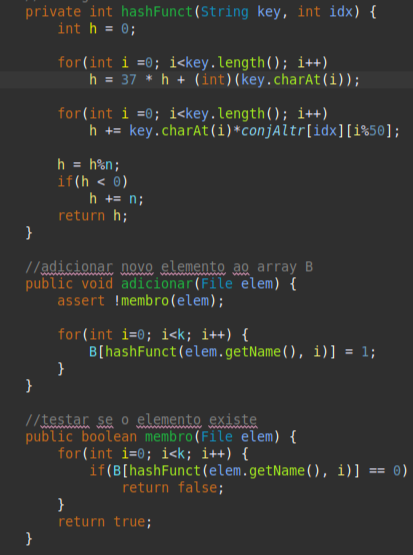
\includegraphics[height=280pt]{methods.png}
\caption{Métodos da classe BloomFilter}
\label{fig:Fig21}
\end{figure}

\subsection{MinHash}

A classe MinHash foi desenvolvida com o intuito de verificar a similaridade entre ficheiros. Tem como atributos uma LinkedList de Strings que serve para guardar os Shingles, um array de Strings para as assinaturas do conjunto, um ficheiro, (o que será futuramente introduzido), dois inteiros (dimensão dos shingles e número de hashFunctions necessárias) e um array bidimensional de inteiros aleatórios que são associados a cada hashFunction.

O construtor da classe, inicializa LinkedList de Shingles e o array com assinaturas do conjunto. É lido o conteúdo do ficheiro que posteriormente vai ser separado em Shingles e comparado. O tamanho dos Shingles varia conforme o tamanho do ficheiro, 5 se este tiver menos de 1000 caracteres e 10 se tiver mais de 1000.

O método {\itshape hashShingle()} retorna o resto da divisão do somatório de todos os Chars (representados pelo seu respectivo código ASCII) de um Shingle, multiplicados por um número aleatório gerado na classe ArrayGenerator. Representa o processo de hash a um Shingle.

{\itshape minHashArray()} passa todos os Shingles por uma função de hash (corresponde a uma posição do array), e o menor valor fica guardado nessa posição. Assim sendo no fim deste processo vamos ter o array de assinaturas preenchido e pronto para comparar com outro com o intuito de obter a similaridade.

{\itshape jaccard()} compara os Shingles presentes em dois arrays de assinaturas de dois conjuntos (dois ficheiros) e devolve o resultado da divisão entre o número de vezes em que os Shingles eram iguais nas mesmas posições do array e o tamanho do array, ou seja calcular a similaridade de jaccard.

\begin{figure}[h]
\center % Centra as imagens
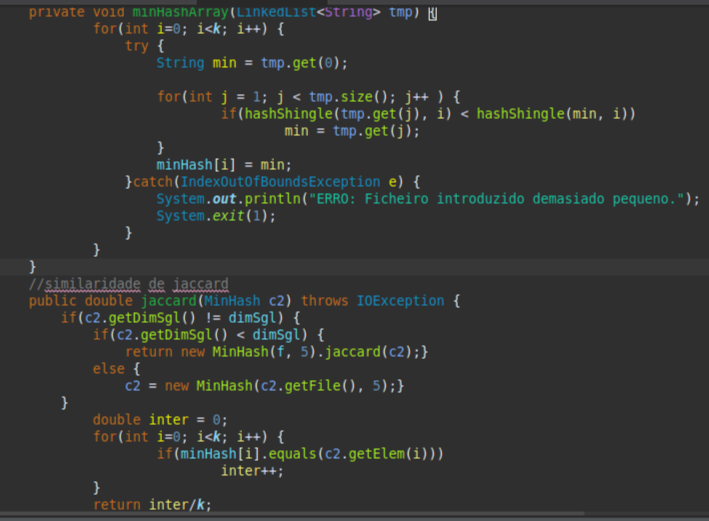
\includegraphics[height=280pt]{min.png}
\caption{Métodos minHashArray e jaccard da classe MinHash}
\label{fig:Fig223}
\end{figure}


\section{Aplicação}
\subsection{GitSystem}
A classe GitSystem tem como atributos uma LinkedList e um BloomFilter e vai servir no geral para gerir os ficheiros introduzidos ou removidos no sistema. O seu uso geral verifica-se na ligação com a janela principal em que cada método é chamado ao premir de botões.

O seu construtor inicia a LinkedList de ficheiros como vazia. Os seus métodos realizam operações tanto sobre a LinkedList como sobre o BloomFilter.
\subsubsection{addFile}
Método que devolve um inteiro de acordo com o resultado da operação realizada e recebe como argumento um ficheiro. A função verifica se o ficheiro já pertence ou não ao BloomFilter e verifica também a similaridade entre os ficheiros para sinalizar na janela principal se for esse o caso. 

Ao pressionar este botão vai ser aberta uma nova {\itshape JFrame} com uma pequena caixa de texto e um botão que permitem enviar um ficheiro ao sistema. O sistema irá sinalizar se o ficheiro não existe, ou se foi adicionado com sucesso, ou se já tinha sido adicionado anteriormente(pertença ao BloomFilter), ou se existem outros ficheiros com conteúdo similar(através da MinHash).

A função devolve:
\begin{itemize}
   \item 0 - Caso de sucesso;
   \item 1 - O ficheiro não existe;
   \item 2 - O ficheiro pertence ao BloomFilter;
   \item 3 - Existem ficheiros similares no sistema.
\end{itemize}

\begin{figure}[h]
\center % Centra as imagens
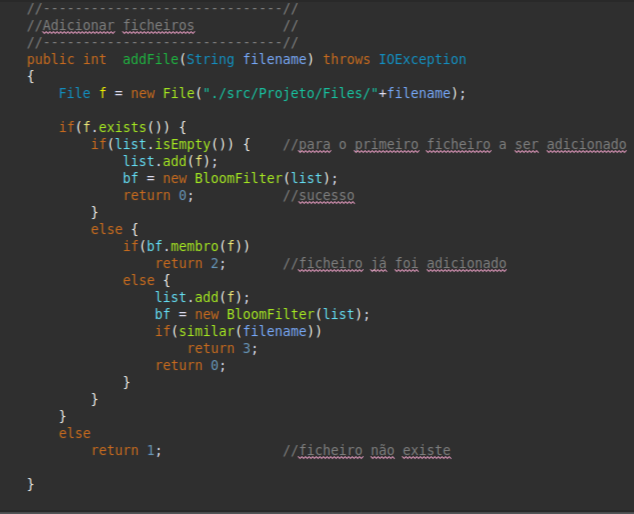
\includegraphics[height=180pt]{add.png}
\caption{Função addFiles}
\label{fig:Fig22}
\end{figure}
 
 Sempre que um ficheiro for adicionado com sucesso ao sistema significa que este foi adicionado à LinkedList que posteriormente foi usada para criar um novo BloomFilter com todos os ficheiros já adicionados.
 
 Para verificar a similaridade o método usa uma função auxiliar ({\itshape similar()}) que devolve true se um ficheiro tiver uma percentagem de similaridade maior ou igual a que 50\%.
 
 
 \subsubsection{removeFile e searchFile}
 Ambas estas funções recebem como argumento um nome de um ficheiro e ambas vão verificar se o mesmo existe no BloomFilter. Se ele existir a removeFile vai removê-lo tanto do BloomFilter como da LinkedList que contem os ficheiros e devolver true, já a função searchFile irá devolver uma String composta pelo conteúdo do ficheiro para posterior apresentação ao utilizador.
 
 \subsubsection{searchSimilarFiles}
 Este método recebe como argumento um ficheiro e vai devolver uma String com a percentagem de similaridade entre o mesmo e todos os ficheiros adicionados ao sistema. Para esse efeito usa o método da descrito anteriormente da MinHash intitulado {\itshape jaccard()} que devolve a similaridade de jaccard entre dois ficheiros.

\begin{figure}[h]
\center % Centra as imagens
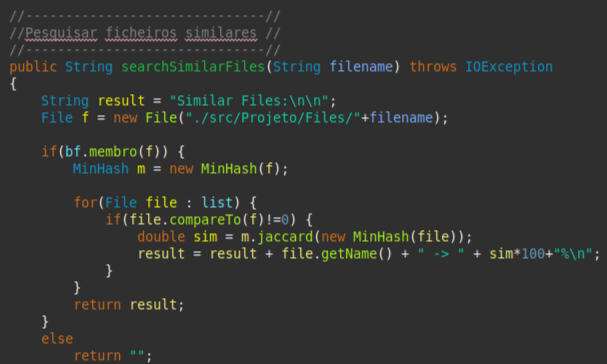
\includegraphics[height=160pt]{ffd.png}
\caption{Função searchSimilarFiles}
\label{fig:Fig23}
\end{figure}

Caso o ficheiro não exista no sistema a função devolve uma String vazia para auxiliar na posterior sinalização dessa ocorrência. 

\subsection{GitWindow}
Esta classe serve maioritariamente para implementação da interface gráfica da aplicação que é descrita mais à frente neste mesmo documento. A GitWindow usa também a classe GitSystem para implementar todas as operações do sistema ao que são executadas quando o utilizador selecciona os botões. Através desta classe são processadas todas as acções do sistema desde inserir ficheiros até à sinalização de erros e apresentação de informação ao utilizador. O resultado e descrição da interface encontram-se no \autoref{chap.func}.






\chapter{Testes}
\label{chap.test}

\section{BloomFilterTeste}
O teste do BloomFilter baseia-se num processo de procura de falsos positivos. São gerados 1000 ficheiros aleatórios usando a classe {\itshape GeradorAleatorioNomes} e desses 1000, 500 são adicionados ao BloomFilter. Posteriormente testa-se se os restantes 500 ficheiros pertencem ou não ao BloomFilter, tendo em conta que estes não foram adicionados. 

Se algum destes últimos 500 que não foram adicionados for membro significa que estamos na presença de um falso positivo. Logo sendo assim todos os falsos positivos vão ser contados.

Este processo vai ser repetido 100 vezes e no fim será calculada a média dos falsos positivos.

O valor obtido deverá estar próximo do valor da probabilidade de falsos positivos, no entanto este não é o caso. Foi obtido um valor muito superior ao esperado visto que o valor definido na classe é 0.01.

\begin{figure}[h]
\center % Centra as imagens
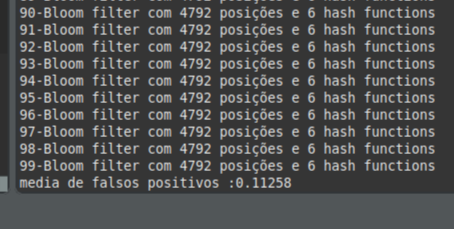
\includegraphics[height=80pt]{pfn.png}
\caption{Resultado do Teste ao BloomFilter}
\label{fig:Fig31}
\end{figure}

Devido à imprecisão deste e de outros testes efectuados(foi procurado um valor que ocupasse a menor memória possível e que apresentasse poucos falsos positivos), foi dificultada a procura do valor da probabilidade de falsos positivos perfeito. O valor apresentado é imperfeito.

\section{MinHashTeste}

O Teste da MinHash consiste no cálculo da similaridade real de dois ficheiros e comparar o valor obtido com o que a classe devolve.

O valor da similaridade real obtém-se através da razão entre o número de shingles iguais entre dois ficheiros o número total de shingles. Logo utilizando dois ficheiros de teste e extraindo os shingles dos mesmos é-nos permitido calcular a similaridade real. 

Ao termos o valor real resta-nos apenas o aplicar o método da classe e comparamos os dois valores. O resultado esperado seria de grande similaridade entre os dois valores.

Ao executarmos o programa vamos obter o resultado especificado na 
\autoref{fig:Fig32}.

\begin{figure}[h]
\center % Centra as imagens
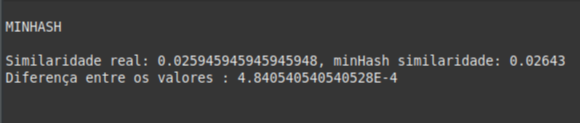
\includegraphics[height=60pt]{MinHash.png}
\caption{Resultado do Teste à MinHash}
\label{fig:Fig32}
\end{figure}

Como podemos verificar a diferença entre os valores é muito pequena o que nos leva a concluir que a procura de similaridade entre ficheiros encontra-se operacional.

\section{Aplicação Conjunta}

Para o teste da aplicação conjunta encontra-se no directório da aplicação uma pasta intitulada de Files que possui uma série de ficheiros prontos a ser usados para o teste.

Alguns dos ficheiros possuem similaridade entre eles o que no irá permitir observar o correto funcionamento da MinHash. Todos os ficheiros pertencem aos autores (possuem conteúdo de outras unidades curriculares) e servem apenas para testar a aplicação conjunta. 

Para testar com ficheiros para além dos que se encontram com a aplicação, seria apenas necessário colocá-los nesse mesmo directório.

O correto funcionamento e descrição da aplicação conjunta pode ser observado no \autoref{chap.func}.





\chapter{Funcionamento}
\label{chap.func}
\section{Janela Principal}

Para observar o funcionamento que irá ser descrito é simplesmente necessário executar o ficheiro {\itshape Main.java}.
\subsection{Interface Gráfica}

A interface gráfica (\autoref{fig:Fig41}) desta aplicação assenta numa {\itshape JFrame} base que suporta outros componentes através dos quais nos apresenta a informação e possibilita o funcionamento do sistema em causa.

Possui três {\itshape JPanels}: um que serve como header para apresentar o título da aplicação, outro para colocação dos botões através dos quais se vai realizar a interacção com a o sistema e finalmente um painel de rodapé.

Esta interface foi desenvolvida e implementada com as ferramentas de {\itshape Java Swing} e derivados.

\begin{figure}[h]
\center % Centra as imagens
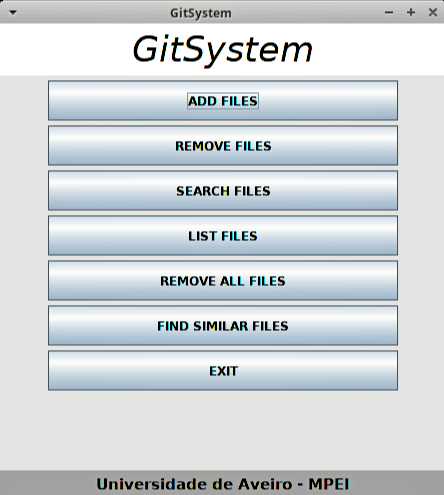
\includegraphics[height=200pt]{MainPage.png}
\caption{Janela Principal da Aplicação}
\label{fig:Fig41}
\end{figure}


\begin{figure}[!tbp]
  \centering
  \begin{minipage}[b]{0.4\textwidth}
    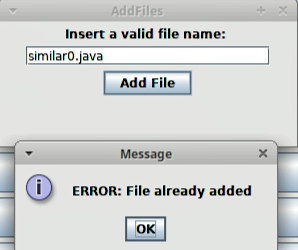
\includegraphics[width=\textwidth]{Addbloom.png}
    \caption{Sinalização de ficheiro já adicionado}
  \end{minipage}
  \hfill
  \begin{minipage}[b]{0.5\textwidth}
    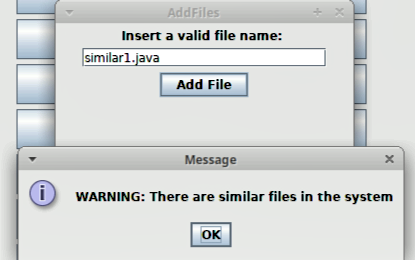
\includegraphics[width=\textwidth]{AddMin.png}
    \caption{Sinalização de ficheiros similares}
  \end{minipage}
\end{figure}

\section{RemoveFiles e SearchFiles}
Ambos estes tal como o anterior ao serem pressionados abrem uma nova janela para que o utilizador possa especificar o ficheiro que pretende que a aplicação use para realizar a ação necessária.

Ambos vão sinalizar o inserir nome de ficheiros inválidos, ou outras situações plausíveis de erro. 

\section{ListFiles e RemoveAllFiles}

Ao serem pressionados, ListFiles imprime o nome de todos os ficheiros adicionados até ao momento ou sinaliza que ainda não foram adicionados se for esse o caso, enquanto que RemoveAllFiles remove todos os ficheiros do sistema e apresenta uma mensagem a indicar esse acto. 

\begin{figure}[!tbp]
  \centering
  \begin{minipage}[b]{0.4\textwidth}
    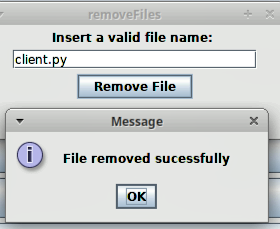
\includegraphics[width=\textwidth]{rmvFiles.png}
    \caption{Sinalização de ficheiro removido}
  \end{minipage}
  \hfill
  \begin{minipage}[b]{0.49\textwidth}
    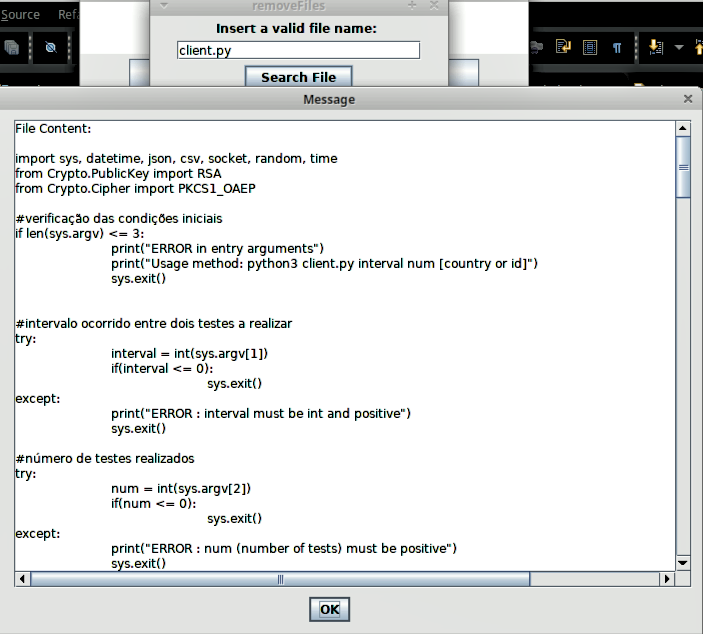
\includegraphics[width=\textwidth]{srchFile.png}
    \caption{Apresentação do conteúdo de um ficheiro (pesquisa)}
  \end{minipage}
\end{figure}

\section{FindSimilarFiles}
Ao ser pressionado este botão apresenta-nos uma nova janela na qual é possível pesquisar um ficheiro. Se este for válido vai-nos ser apresentada uma lista contento os ficheiros adicionados e a percentagem de similaridade de cada um destes com o ficheiro pesquisado.

\begin{figure}[h]
\center % Centra as imagens
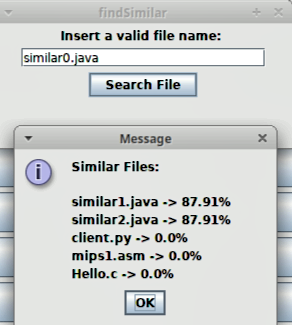
\includegraphics[height=130pt]{simila.png}
\caption{Similaridade entre ficheiros}
\label{fig:Fig46}
\end{figure}


\chapter{Conclusões}
\label{chap.conclusao}

A base da aplicação funciona, ou seja foi implementado um sistema do tipo Git que permita gerir ficheiros. O sistema sinaliza similaridade entre ficheiros e impede o utilizador de inserir ficheiros com nomes iguais.

Apesar de o módulo do BloomFilter estar a funcionar correctamente na aplicação conjunta, concluímos a partir dos testes efectuados que este apenas opera bem para poucas quantidades de ficheiros, ou seja se fossem inseridas grandes quantias a probabilidade de adição de ficheiros com nomes iguais aumentaria muito mais. Logo constata-se que este módulo não está nas melhores condições.

O módulo da MinHash funciona correctamente como foi demonstrado nos testes. Ao adicionar ficheiros à aplicação também se verificou uma execução correta desta classe que também é visivel quando se pesquisa por ficheiros similares.

\chapter{Contribuições dos autores}
Este projeto foi realizado por \ac{jg} e \ac{mr}.
Ambos os autores contribuíram igualmente para o trabalho tanto na discussão do projeto, como no desenvolvimento do mesmo. 

%%%%%%%%%%%%%%%%%%%%%%%%%%%%%%%%%
\chapter*{Acrónimos}
\begin{acronym}
\acro{jg}[JG]{João Gameiro}
\acro{mr}[MR]{Marco Ramos}
\acro{mpei}[MPEI]{Métodos Probabilísticos para Engenharia Imformática}
\acro{ect}[ECT]{Engenharia de Computadores e Telemática}
\end{acronym}


%%%%%%%%%%%%%%%%%%%%%%%%%%%%%%%%%
\printbibliography

\end{document}